\documentclass[xcolor=dvipsnames, aspectratio=169]{beamer} 

\mode<presentation> {
	%\usetheme{Singapore}
	%\usetheme{CambridgeUS}
	\usecolortheme{dolphin}
	\definecolor{anti-flashwhite}{rgb}{0.95, 0.95, 0.96}
	\definecolor{lightgray}{rgb}{0.83, 0.83, 0.83}
	\setbeamercolor{block title}{use=structure,fg=black,bg=RoyalPurple!60}
	\setbeamercolor{block body}{use=structure,fg=black,bg=RoyalPurple!10}
	\setbeamercolor{block title example}{fg=black,bg=RoyalPurple!20}
	\setbeamercolor{block body example}{fg=black,bg=RoyalPurple!5}
	\definecolor{darkred}{rgb}{0.8,0,0}
	\setbeamercolor*{item}{fg=DarkOrchid}
}

%\lstdefinestyle{mystyle}{
%	basicstyle=\tiny,
%	%backgroundcolor=\color{backcolour},   
%	%commentstyle=\color{codegreen},
%	keywordstyle=\color{blue},
%	%numberstyle=\tiny\color{codegray},
%	%stringstyle=\color{codepurple},
%	breakatwhitespace=false,         
%	breaklines=true,                 
%	captionpos=b,                    
%	keepspaces=true,                 
%	numbers=left,                    
%	numbersep=5pt,                  
%	showspaces=false,                
%	showstringspaces=false,
%	showtabs=false,                  
%	tabsize=2,
%	%aboveskip=2em,
%	%belowskip=2em
%}
	
%Packages
\usepackage{graphicx}
\usepackage[english]{babel}
\usepackage[utf8]{inputenc}
\usepackage{amsmath, amsfonts, amssymb}
\usepackage{paralist}
\usepackage{mathtools}

\usepackage{lmodern}
%\usepackage{MnSymbol}

\usepackage{tabularx}
\usepackage{ragged2e} 
\usepackage{enumerate}
\usepackage{bbm}
\usepackage{bbold}
\usepackage{pgfplots}
\usepackage{tikz}
\usetikzlibrary{fit,calc,positioning,decorations.pathreplacing,matrix}
\usepackage{calligra}
\usepackage{graphicx}
\usepackage{subfigure}
\usepackage{caption}
\usepackage[bottom]{footmisc}
\usepackage{multimedia}
\usepackage{csquotes}
\usepackage[backend=biber, natbib=true, style=numeric]{biblatex}
\addbibresource{refs.bib}
\usepackage{hyperref}
\usepackage{listings}
\usepackage{transparent}
%\usepackage{natbib}
\usepackage{bibentry}
\usepackage{filecontents}
%\usepackage[style=verbose,backend=bibtex]{biblatex}

\usepackage{xcolor}

%\usepackage{enumitem}

%MOVIES
\usepackage{animate}
\usepackage{media9}

%vertical writing
\newcommand{\btVFill}{\vskip0pt plus 1filll}

% the copyright
\usepackage{txfonts}

%brackets
%\usepackage{amsmath}
%\usepackage[clean]{svg}




\newtheorem{conjecture}{Conjecture}


%TITLE PAGE

\title{Vergleich zwischen makro- und mikroskopischen Verhalten des Random Walk im Kontext von Size-Exclusion}
\author{Aaron Pumm}
\institute{Universität Wien}
%\addtobeamertemplate{title page}{}{joint work with ...} 
\logo{
\includegraphics[scale=0.2]{Uni_Logo_2016.jpg}}%~\includegraphics[scale=0.05]{logo_sfb_blue.jpg}}


\date{12.01.2023 \\ \vspace{0.2in} \footnotesize{Betreuer: \textit{Michael Fischer} (Universität Wien)}}



\AtBeginSection[]
{
	\begin{frame}[t]
		\frametitle{Inhalt}
		\tableofcontents[currentsection]
	\end{frame}
}

\makeatletter
%\setbeamertemplate{footline}
%{
%	\leavevmode%
%	\hbox{%
%		\begin{beamercolorbox}[wd=.25\paperwidth,ht=2.25ex,dp=1ex,left]{author in head/foot}%
%			\usebeamerfont{author in head/foot}\hspace*{2em}\insertshortauthor
%		\end{beamercolorbox}%
%		\begin{beamercolorbox}[wd=.5\paperwidth,ht=2.25ex,dp=1ex,center]{title in head/foot}%
%			\usebeamerfont{title in head/foot} DEA 2019, AGH University of Science and Technology%\insertsection %\insertsubsection
%		\end{beamercolorbox}%
%		\begin{beamercolorbox}[wd=.25\paperwidth,ht=2.25ex,dp=1ex,right]{date in head/foot}%
%			\usebeamerfont{date in head/foot} September 20, 2019\hspace*{2em}%\insertshortdate{}
%			%\insertframenumber{} / \inserttotalframenumber\hspace*{2ex}
%		\end{beamercolorbox}}%
%		\vskip0pt%
%	}
%	\makeatother 
	

\begin{document}
\nocite{*}

\begin{frame}[t]
	\titlepage
\end{frame}

\logo{}

%contents
%\begin{frame}[t]
%\frametitle{Table of Contents}
%\tableofcontents % [paussections]
%\end{frame}

%slides


\section{Motivation}

\begin{frame}{Motivation}
	\begin{minipage}{0.3\linewidth}
        \begin{itemize}
            \item Messe
            \item Fahrstuhl
            \item Stadion
            \item Rolltreppen
        \end{itemize}
    \end{minipage}
    \begin{minipage}{0.69\linewidth}
    % Rechte Spalte mit Grafik.
        \begin{center}
            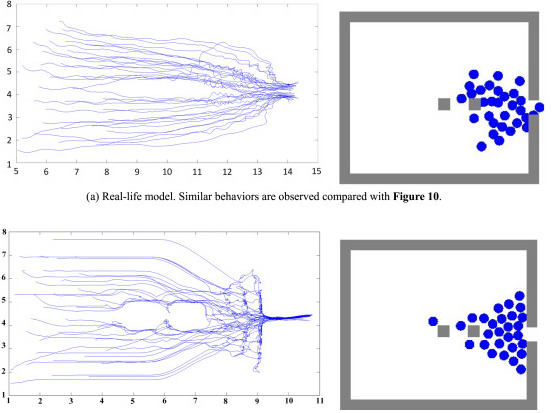
\includegraphics[width=\linewidth]{figures/pedestrianMovement.jpg}
        \end{center}
        \cite*{song2018data}
    \end{minipage}
\end{frame}

%\begin{frame}{The cellular automaton}
%	\center
%	\begin{tikzpicture}
%	[help lines/.style={draw=black},
%	every node/.style={help lines,rectangle,minimum size=3mm},
%	cellular automaton/.style={draw=none,row sep=0mm,column sep=0mm, ampersand replacement=\&},
%	rst/.style={fill=white,help lines},
%	exc/.style={fill=blue!70,help lines}
%	ref/.style={fill=blue!30!white,help lines}]
%	
%		\matrix[cellular automaton] {
%			\node[rst] {};\& \node[rst] {};\& \node[rst] {}; \\
%			\node[rst] {};\& \node[exc] {};\& \node[rst] {}; \\
%			\node[rst] {};\& \node[rst] {};\& \node[rst] {}; \\
%		};
%	\end{tikzpicture}
%\end{frame}
\section{Modelle und Skalen}

\begin{frame}[t]{Mikroskopisches modellieren}

\begin{exampleblock}{Definition}
    Ein Modell auf mikroskopischer Ebene simultiert das detailierte Verhalten des zu betrachteneden Systems und es lassen sich genaue Wechselwirkungen zwischen den untersuchten Objekten feststellen. 
\end{exampleblock}
\pause
Beispiele für solche Größen wären: 
\vspace{5mm}
\begin{itemize}
\setlength\itemsep{1em}
    \item<2-> Trajektorien von einzelnen Agenten oder Partikeln $x_i$
    \item<3-> Geschwindigkeit $v_i$
    \item<4-> ODEs, SDEs, zellulare Automaten
\end{itemize}
\end{frame}

\begin{frame}[t]{Makroskopisches modellieren}
\begin{exampleblock}{Definition}
    Ein Modell auf makroskopischer Ebene beschreibt lediglich das Verhalten des gesamten Systems und einzelne Effekte, die nicht sichtbar zum Verhalten des Systems beitragen werden häufig vernachlässigt oder lassen sich nicht extrahieren. 
\end{exampleblock}
\pause
Beispiele für solche Größen wären: 
\vspace{5mm}
\begin{itemize}
\setlength\itemsep{1em}
    \item<2-> Dichte $\rho(t)$ einer Menschenmenge
    \item<3-> Potentiale oder Kurven
    \item<4-> Anteil eines Stoffes im Blut
\end{itemize}
\end{frame}

\section{Random Walk}
\begin{frame}{Random Walk}
\begin{exampleblock}{Definition}
Der Random Walk ist ein stochastischer Prozess der die Trajektorie $x_i(t)$ eines Agenten $i$ durch die Abfolge von zufälligen Schritten, die innerhalb einer vorgegebenen Umgebung liegen, beschreibt.  
\end{exampleblock}
\end{frame}
\begin{frame}[t]{Random Walk Umgebungen}
	\begin{center}
		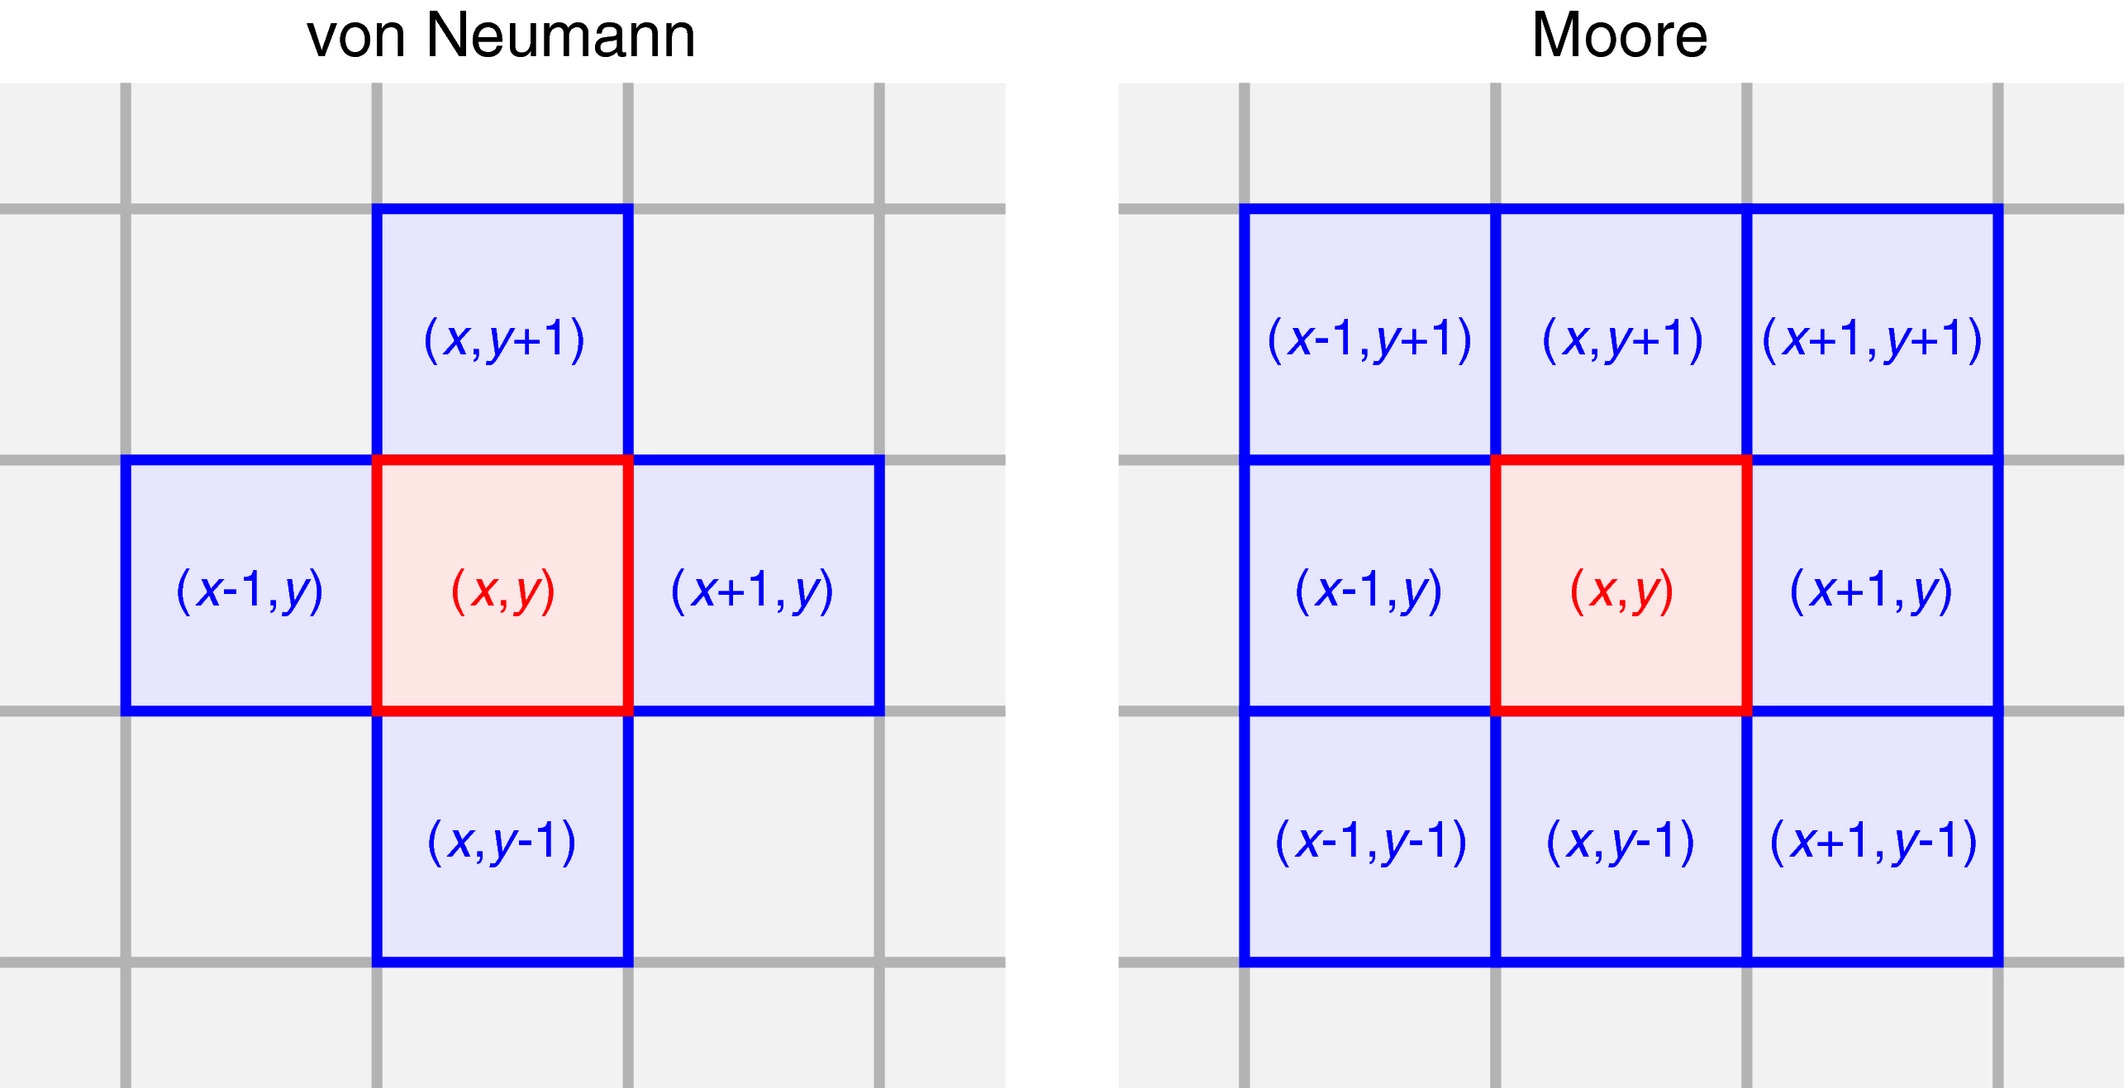
\includegraphics[width=0.8\linewidth]{figures/CA_Umgebungen.png} 
	\end{center}
\end{frame}

\begin{frame}{Mastergleichung}
\begin{exampleblock}{Zellulärer Automat als mathematische Gleichung}
    \begin{equation}
        \begin{split}
        \rho(x,t+\Delta t) - \rho(x,t) & =  - \rho(x,t)\mathcal{T}^{+}(x,t) - 
        \rho(x,t)\mathcal{T}^{-}(x,t) \\  & + \rho(x +\Delta x,t)\mathcal{T}^{-}(x + \Delta x,t) + \rho(x -\Delta x,t)\mathcal{T}^{+}(x - \Delta x,t) 
        \end{split}
    \end{equation}
    mit $\rho \in \{0,1\}$ die Dichte in Zeit $t$ und Position $x$
\end{exampleblock}
\begin{itemize}
    \item Übergangsrate $\mathcal{T}$ konstant führt zu Random Walk 
    \item kann auch komplexer gewählt werden für umfangreichere Dynamiken 
    \\(z.B. Size Exclusion)
\end{itemize}
\end{frame}

\begin{frame}{Size Exclusion}
    Size Exclusion als zusätzliche Vorsschrift für Verhalten von Random Walk Agenten
    \vspace{5mm}
    \\
    zwei Agenten nicht in das selbe Feld zur selben Zeit
    \vspace{5mm}
    \\
    kann im Sinne der Mastergleichung durch einen Term $(1-\rho(x,t))$ in $\mathcal{T}$ modelliert werden
    \\
    \vspace{5mm}
    \begin{center}
       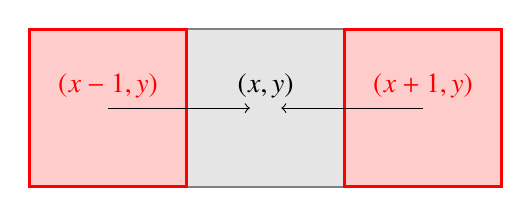
\begin{tikzpicture}
        \filldraw [fill=gray!20, draw=gray, thick] (2, 0) rectangle +(2, 2);
        \filldraw [fill=red!20, draw=red, very thick] (0, 0) rectangle +(2, 2);
        \filldraw [fill=red!20, draw=red, very thick] (4, 0) rectangle +(2, 2);
      
        \draw [->] (5, 1)node[above,color=red]{$(x+1, y)$} -- (3.2, 1);
        \draw [->] (1, 1)node[above,color=red]{$(x-1, y)$} -- (2.8, 1);
        \draw node[above] at (3, 1) {$(x, y)$};           
    \end{tikzpicture} 
    \end{center}
\end{frame}

\section{Numerische Simulationen}

\begin{frame}{Random Walk}

Reihenfolge für das updaten der Agenten ist relevant
\vspace{5mm}
\begin{itemize}
\setlength\itemsep{1em}
    \item <2-> sequentielles updaten
    \item <3-> Reihenfolge der Agenten mischen
    \item <4-> paralleles updaten (Konflikt Lösung) 
\end{itemize}
    
\end{frame}

\begin{frame}{Random Walk}

    Reihenfolge für das updaten der Agenten ist relevant
    \vspace{5mm}
    \begin{itemize}
    \setlength\itemsep{1em}
        \item sequentielles updaten
        \item Reihenfolge der Agenten mischen
        \item paralleles updaten (Konflikt Lösung) 
    \end{itemize}
    \vspace{5mm}
    Für die Simulationen werden periodische Randbedingungen verwendet.
        
\end{frame}

\begin{frame}[t]{Random Walk}
\begin{center}
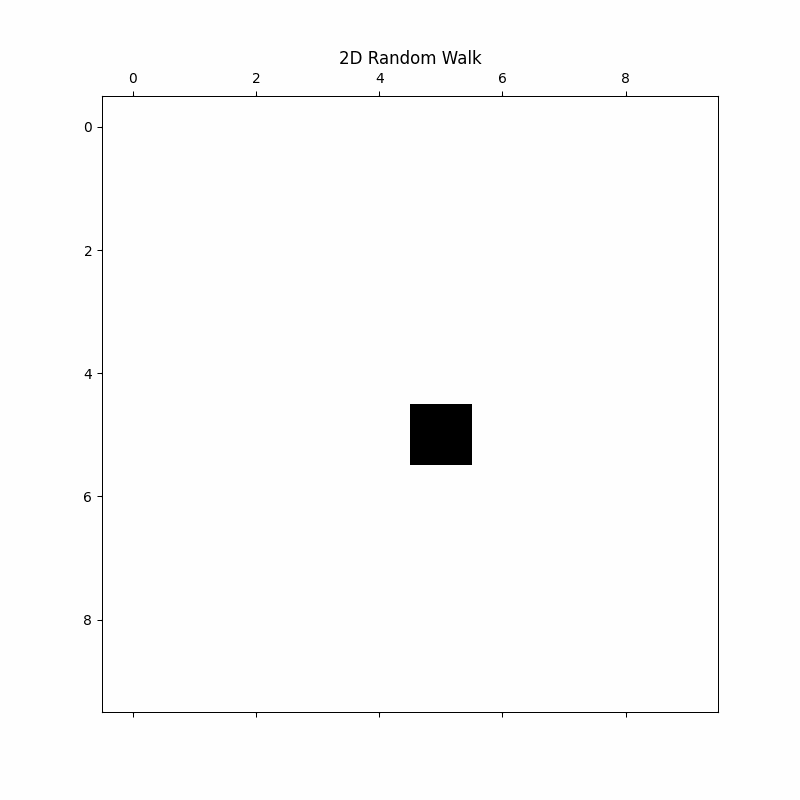
\includegraphics[width=0.5\linewidth]{figures/RW/RW-0.png} 
\end{center}
\end{frame}

\begin{frame}[t]{Random Walk}
\begin{center}
\animategraphics[autoplay,width=0.5\linewidth]{4}{figures/RW/RW-}{0}{25}
\end{center}
\end{frame}

\begin{frame}{Random Walk mit mehreren Agenten}
\begin{center}
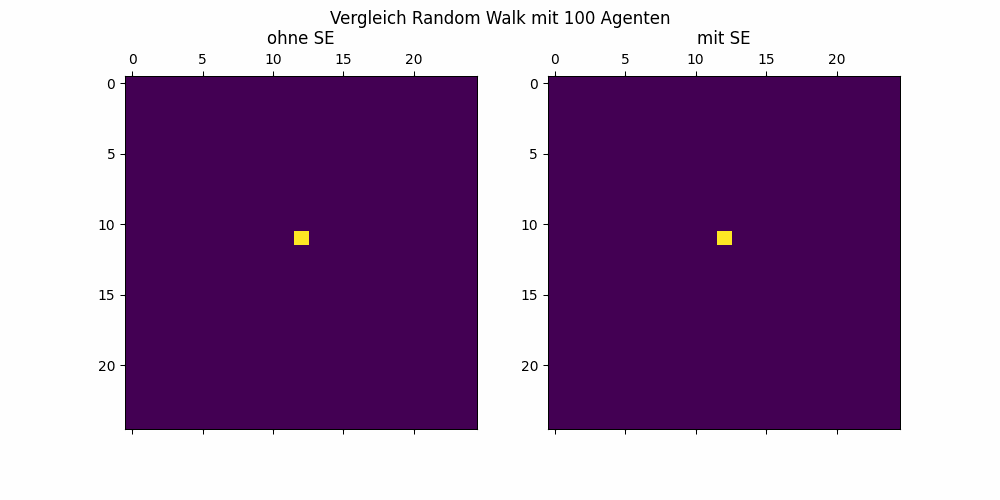
\includegraphics[width=0.7\linewidth]{figures/VergleichRW_SE/VergleichRW_SE-0.png} 
\end{center}
\end{frame}

\begin{frame}{Random Walk mit mehreren Agenten}
\begin{center}
\animategraphics[autoplay,width=0.7\linewidth]{10}{figures/VergleichRW_SE/VergleichRW_SE-}{1}{198}
\end{center}
\end{frame}


\begin{frame}{Monte Carlo Simulationen in 1D}
\begin{center}
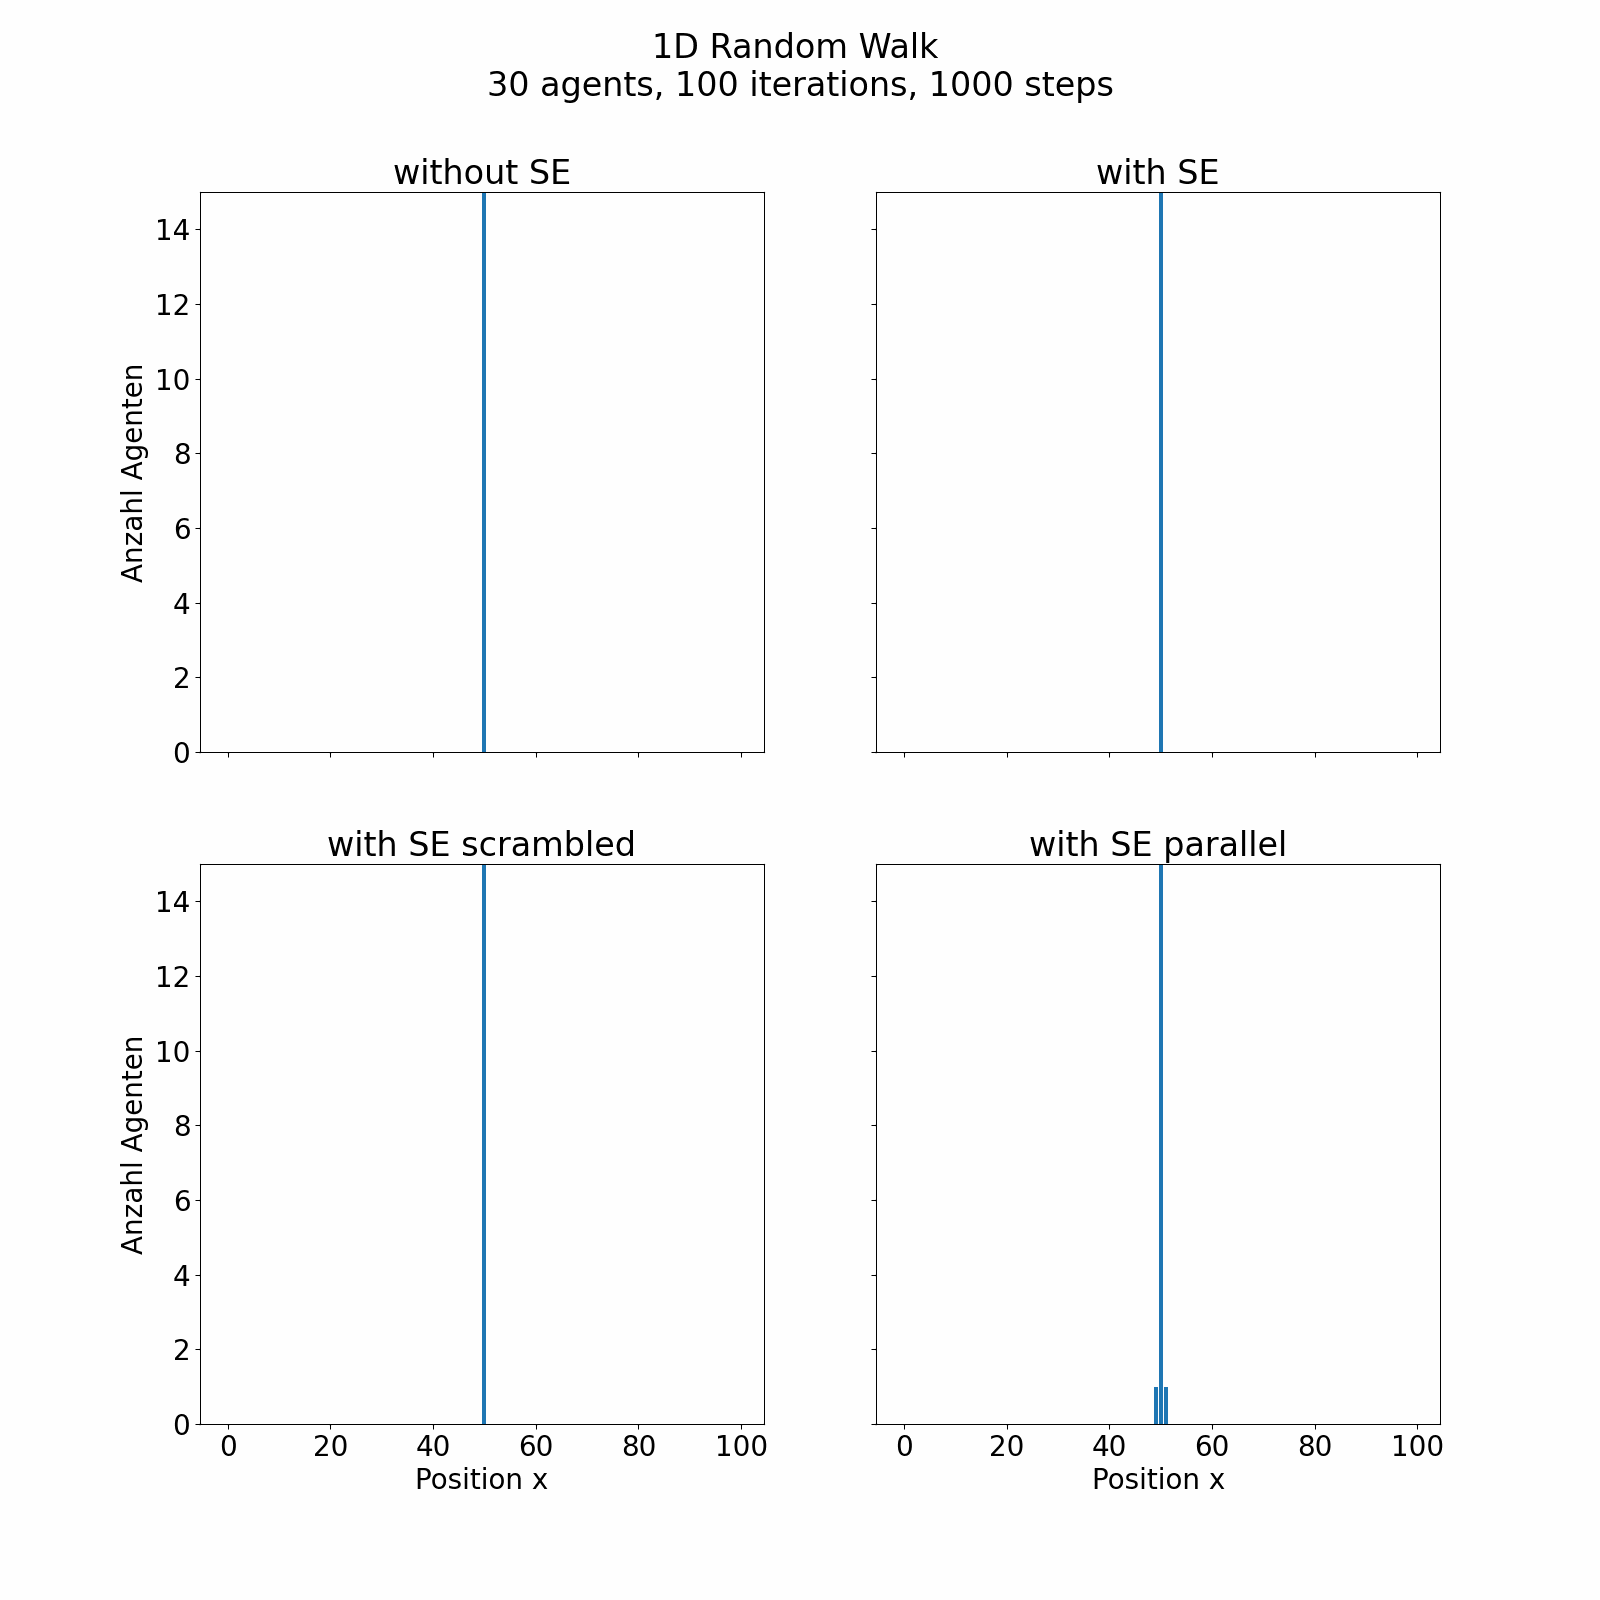
\includegraphics[width=0.45\linewidth]{figures/Vergleich4/Vergleich4-0.png} 
\end{center}
\end{frame}

\begin{frame}{Monte Carlo Simulationen in 1D}
\begin{center}
\animategraphics[autoplay,width=0.45\linewidth]{10}{figures/Vergleich4/Vergleich4-}{1}{198}
\end{center}
\end{frame}

\begin{frame}{Herleitung der PDE}[t]
    Wir wollen aus der Mastergleichung eine PDE herleiten für das makroskopische Verhalten.
    Wählen wir $\mathcal{T}$ konstant $ \frac{1}{3}$ resultiert die Mastergleichung in dem Random Walk.
\begin{equation}
    \rho(x,t+\Delta t) - \rho(x,t)  =  \frac{1}{3} (\rho(x + \Delta x, t) - 2 \rho(x,t) + \rho(x - \Delta x, t))
\end{equation}
    Nimmt man genügend Regularität an $\rho$ an kann man es durch seine Taylorreihenentwicklung ersetzen
\pause
\begin{equation}
    \rho(x, t + \Delta t) = \rho(x, t) + \Delta t \frac{\partial}{\partial t}\rho(x, t) + O(\Delta t)^2
\end{equation}
\begin{equation}
    \rho(x + \Delta x, t) = \rho(x, t) + \Delta x \frac{\partial}{\partial x}\rho(x, t) + \frac{1}{2}(\Delta x)^2 \frac{\partial^2}{{\partial x}^2}\rho(x,t) + O(\Delta t)^3
\end{equation}
\end{frame}

\begin{frame}{Herleitung der PDE}
    Ersetzt man diese Terme in der Mastergleichung und setzt $\frac{\Delta t}{(\Delta x)^2}$ konstant erhält man für $\Delta t \rightarrow 0$:
    \begin{equation}
        \partial_t \rho (x,t) = \frac{1}{3} \partial_{x x} \rho(x,t)
    \end{equation} 
    Was der Wärmleitgleichung entspricht welche eine explizite Lösung besitzt
\end{frame}

\begin{frame}[t]{Diskretisierung der Heat Equation}

    Wir approximieren die Zeitableitung mit der Vorwärtsdifferenz: 
    \begin{equation}
        \partial_t \rho(x_j,t_n) \approx  \frac{U^{n+1}_j-U^{n}_j}{\Delta t}
    \end{equation}
    Wir approximieren die Ortsableitung mit der Zentraldifferenz zweiter Ordnung: 
    \begin{equation}
        \partial_{xx} \rho(x_j,t_n) \approx  \frac{U^{n}_{j-1}-U^{n}_j+U^{n}_{j+1}}{{\Delta x}^2}
    \end{equation}
    Eingesetzt in die Differentialgleichung und umgeformt nach $U^{n+1}$ erhält man genau die vorher gezeigte Mastergleichung mit Konstante $\mathcal{T} \sim \frac{\Delta t}{{\Delta x}^2}$  
     
\end{frame}
\begin{frame}{Numerische Lösung der Wärmleitgleichung}
    \begin{center}
        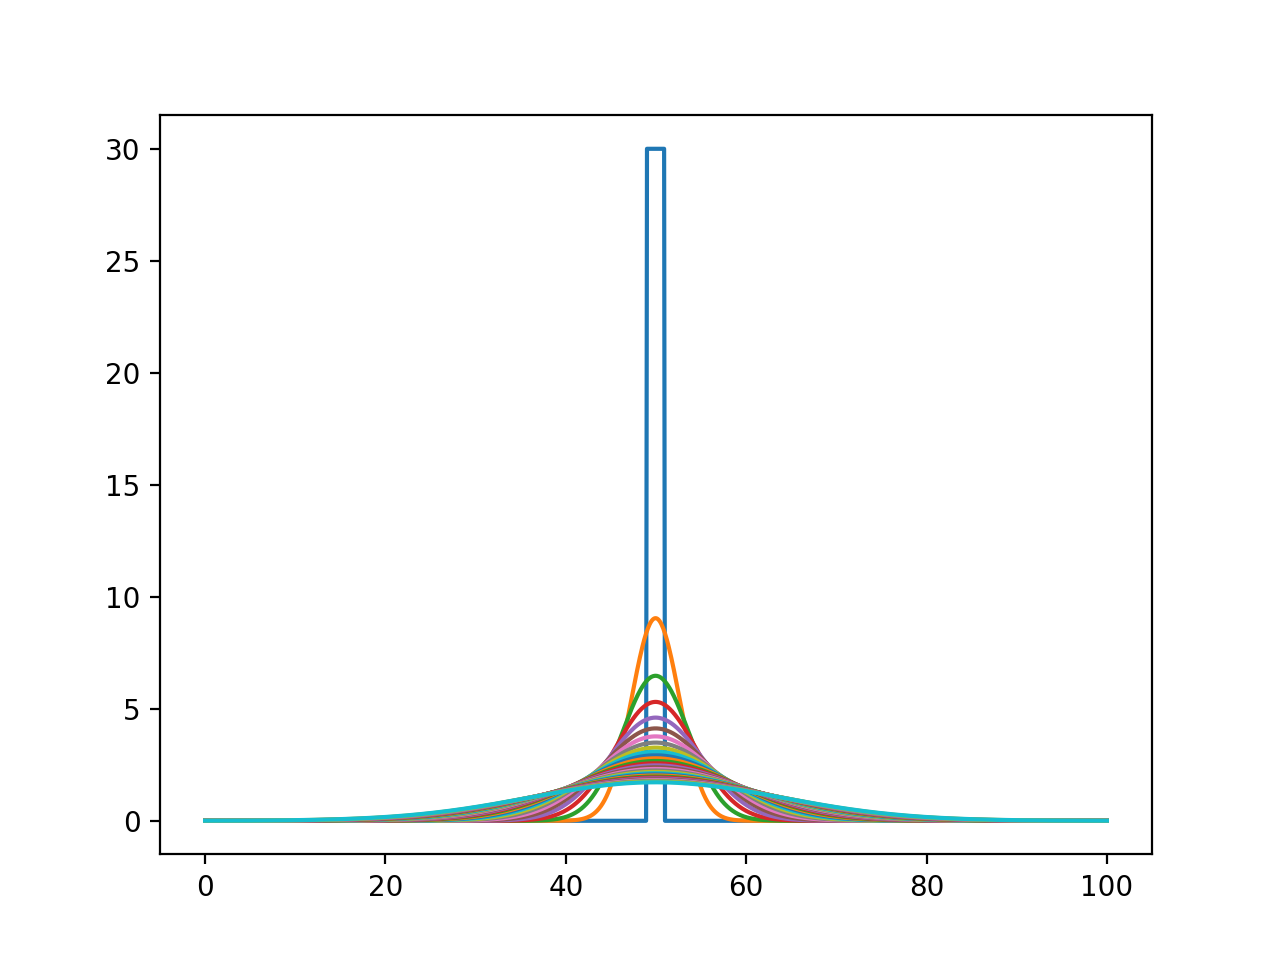
\includegraphics[width=0.7\linewidth]{figures/Heat1Dadjustiert.png} 
    \end{center}
\end{frame}

\begin{frame}
\begin{center}
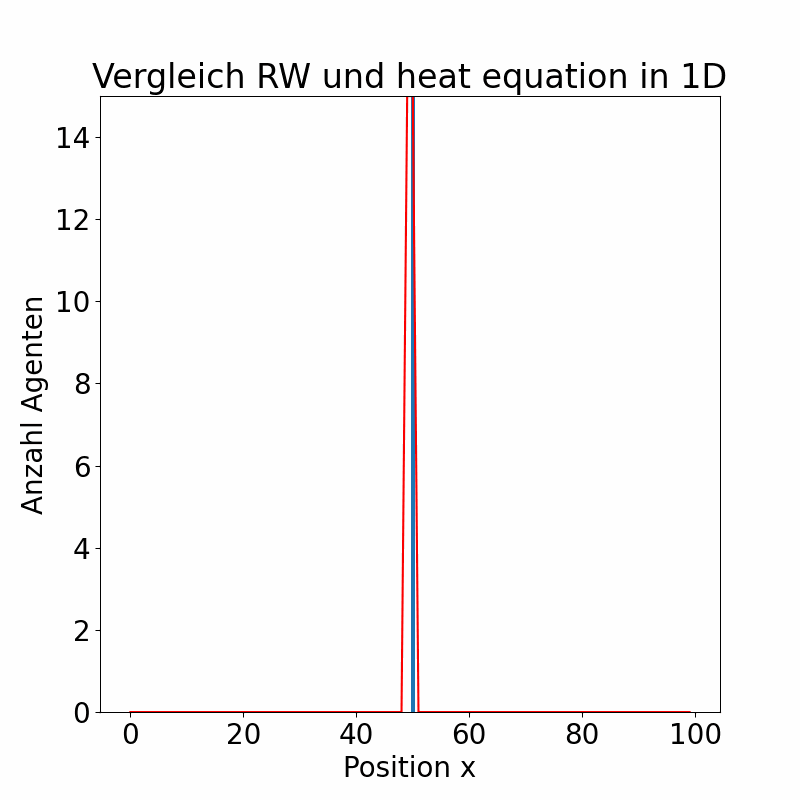
\includegraphics[width=0.45\linewidth]{figures/VergleichRW_Heat/VergleichRW_Heat-0.png} 
\end{center}
\end{frame}

\begin{frame}
\begin{center}
\animategraphics[autoplay,width=0.45\linewidth]{10}{figures/VergleichRW_Heat/VergleichRW_Heat-}{1}{198}
\end{center}
\end{frame}

\begin{frame}
\begin{center}
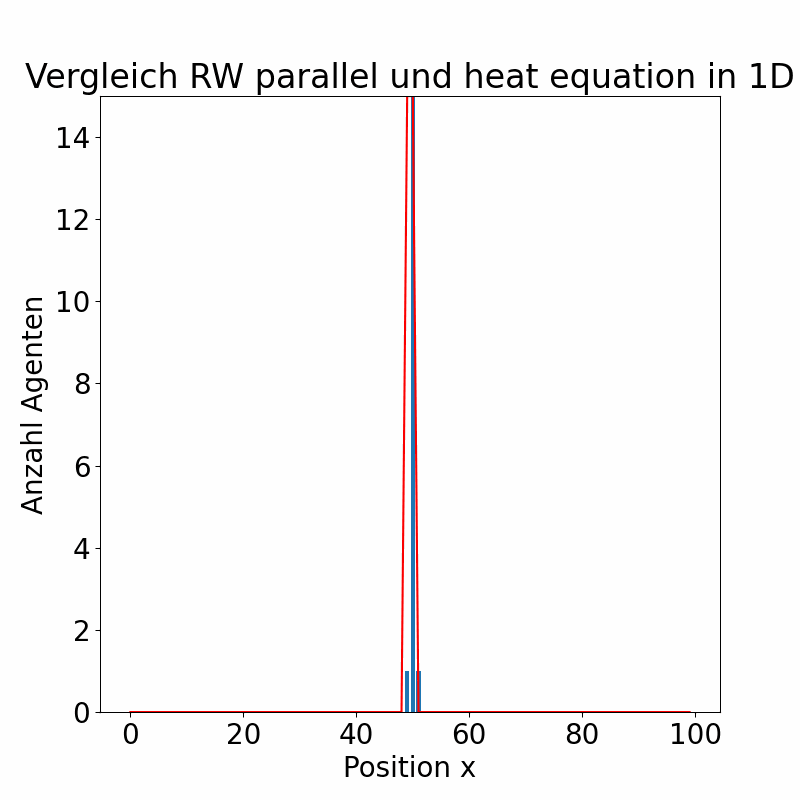
\includegraphics[width=0.45\linewidth]{figures/VergleichRW_SE_Heat/VergleichRW_SE_Heat-0.png} 
\end{center}
\end{frame}

\begin{frame}
\begin{center}
\animategraphics[autoplay,width=0.45\linewidth]{10}{figures/VergleichRW_SE_Heat/VergleichRW_SE_Heat-}{1}{198}
\end{center}
\end{frame}

\section{Interpretation der Resultate}
\begin{frame}
	\begin{itemize}
		\item alle mikroskopischen Modelle verhalten sich unterschiedlich
		\item die hergeleitete PDE verfehlt makroskopisches Verhalten des Random Walks mit Size Exclusion
		\item Vermutung: Masterequation hat keine Konfliktlösung eine andere PDE ist die richtige: 
        \begin{equation}
            \frac{\partial}{\partial t} f(x,t) = \frac{\partial ^{2}}{\partial t ^{2}}  \frac{1}{18} f(x,t) \left(-\mu  f(x,t)^2+\mu  f(x,t)+6\right)
        \end{equation}
	\end{itemize} 
\end{frame}
\begin{frame}{Quellen}
    \printbibliography{}
\end{frame}
\end{document}

%https://onlinelibrary.wiley.com/cms/asset/9840368b-1a80-4463-9d8a-311fba191c69/dneu22686-fig-0001-m.jpg CA Umgebungen